\section{Introduction}
% Problem definition

% extracting intent/meaning from a set of words (more strictly sentences)

\subsection{Data Preprocessing}
Training data was processed by running each sample through a pre-trained deep sentence embedding model to produce a 384 dimensional dense vector. The embedding model used was \verb|all-MiniLM-L12-v2| \cite{HuggingFace} from the \verb|sentence-transformers| library provided by HuggingFace , this was chosen for its strong listed transfer performance and its relatively small size. However, this model is optimised for sentences of 128 words or less and will truncate sentences that are longer than 512 words. Because many of the reviews in the dataset are longer than 512 words this poses an issue. Experiments were performed using tokenisation and stop word removal to reduce sentence length but this severely worsened the performance of the model. Intuitively this makes sense because the embedding model is trained on natural language and assumes input sentences are grammatical. Instead, any reviews longer than 128 words are split into 128 word long chunks which are embedded individually and averaged together. In order to preserve semantic continuity between chunks they overlap by 15 words. Chunks are weighted by length when averaged to account for reviews which are not a multiple of 128 long. This provided a significant improvement in accuracy, approximately 5\%,  over allowing long reviews to be truncated.

Shown in \autoref{fig:feature_corr_hm} you can see the correlation between the features provided  by the embedding method and the sentence sentiment.\\
It is clear that although there does not appear to be any single feature that is positively or negatively correlated to the sentiment, there are several features which are all over 20\% positively or negatively correlated (indicated by the bright yellows and dark blues).\\
You can also find within the appendix \autoref{fig:feature_corr_hm_old}, which shows the same heatmap, but using the embeddings without performing chunking and overlapping, i.e. where sentences where truncated to 128 word items.
\begin{figure}[h]
    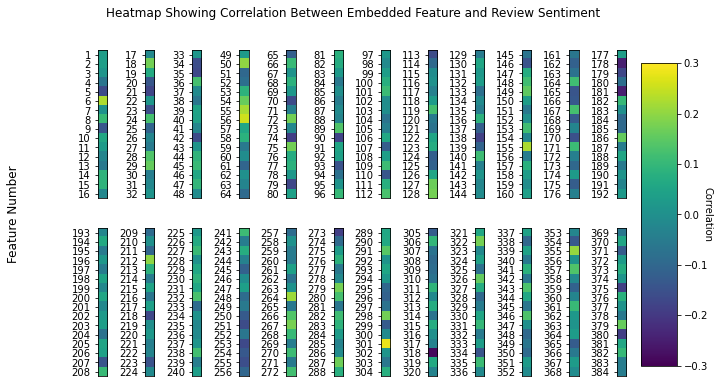
\includegraphics[width=\textwidth]{figures/Feature_Correlation_Heatmap_Non_Trunkated_Embedding.png}
    \caption{\label{fig:feature_corr_hm} Heat-map showing correlation of embedding features to the sentence sentiment}
\end{figure}